\documentclass{fund}
\let\ifpdf\relax % http://tex.stackexchange.com/questions/11414/package-ifpdf-error

%\includeonly{ch01/ch01temp}

\makeindex
\pdfmapfile{=fullembed.map} % created by the script create_fullembed_file

\begin{document}

%\thispagestyle{empty}
\raisebox{0mm}[0mm][0mm]{%
\parbox{8.5in}{
\vspace*{236mm}\hspace{-38.5mm}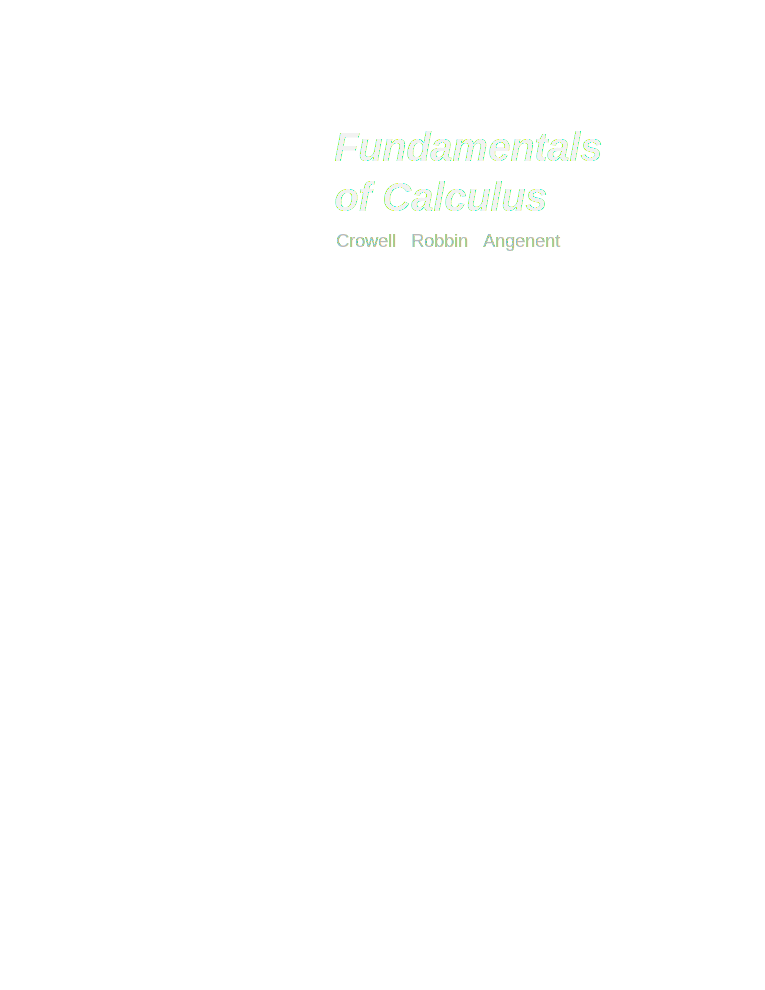
\includegraphics{cover/cover-for-pdf.png}\\
}
}%
\\


\cleardoublepage

\thispagestyle{empty}

\vspace{100mm}

{\sffamily

\noindent {\Huge Fundamentals of Calculus}

\vspace{10mm}

\noindent {\huge Crowell, Robbin, and Angenent}

\vspace{10mm}

\noindent This open-source book by Benjamin Crowell is based upon
a previous open-source book by Joel Robbin and Sigurd Angenent.

\vspace{10mm}

\noindent www.lightandmatter.com

}


\thispagestyle{empty}

\vspace{100mm}

\noindent
\includegraphics{cover/lmlogo}\\
Fullerton, California\\
www.lightandmatter.com

\vspace{20mm}
\noindent
Copyright 2006 Sigurd B.~Angenent, Laurentiu Maxim, Evan Dummit, and Joel Robbin.
Copyright 2014 Benjamin Crowell.
Copyrights of some images are held by other authors; see the photo credits section
at the back of the book.

\vspace{20mm}
\noindent
rev. \today{}

\vspace{6mm}
\noindent
Permission is granted to copy, distribute and/or
modify this document under the terms of the GNU Free Documentation License, Version
1.3 or any later version published by the Free Software Foundation; with no Invariant
Sections, no Front-Cover Texts, and no Back-Cover Texts. A copy of the license is
available at\linebreak[4]
www.gnu.org/copyleft/fdl.html.

For the portions of the book authored by Benjamin Crowell, users may, at their option,
choose to copy, distribute and/or modify it
under the terms of the Creative Commons Attribution
Share-Alike License, which can be found at creativecommons.org.

This book can be downloaded free of charge
from\linebreak[4]
www.lightandmatter.com in a variety of formats,
including editable formats.


\pagebreak\vspace{100mm}

\hbox{}\noindent\huge\bfseries\sffamily{}\hspace{-2mm}\ \ Brief Contents\\
\hspace{-20mm}\noindent\mynormaltype\Large\sffamily{}\begin{tabular}{rl}
\ref{ch:derivative} & An informal introduction to the derivative \quad \pageref{ch:derivative}\\
\ref{ch:limits} &  Limits; techniques of differentiation \quad \pageref{ch:limits}\\
\ref{ch:second-derivative} & The second derivative \quad \pageref{ch:second-derivative}\\
\ref{ch:more-limits} & More about limits; curve sketching\quad \pageref{ch:more-limits}\\
\ref{ch:more-derivatives} & More derivatives\quad \pageref{ch:more-derivatives}\\
\ref{ch:indeterminate-forms} & Indeterminate forms and L'H\^{o}pital's rule 
                  \quad \pageref{ch:indeterminate-forms} \\
\ref{ch:from-functions-to-variables} & From functions to variables
                  \quad \pageref{ch:from-functions-to-variables} \\
\ref{ch:integral} & The integral
                  \quad \pageref{ch:integral} \\
\ref{ch:integration-techniques} & 
                  Basic techniques of integration
                  \quad \pageref{ch:integration-techniques} \\
\end{tabular}
\mynormaltype

\vspace{100mm}\pagebreak

\cleardoublepage

%%%%%%%%\noindent\huge\bfseries\sffamily{}\hspace{-2mm}\ \ Contents\\
\mynormaltype

\tableofcontents

%========================= main matter =========================
\mainmatter
%-- I want the whole book numbered sequentially, arabic:
  \pagenumbering{arabic} 
  \addtocounter{page}{8} 
\parafmt
\myeqnspacing % Do this early and often, since it gets reset by \normalsize
%========================= chapters =========================
	\renewcommand{\chapdir}{ch01}\include{ch01/ch01temp}
	\renewcommand{\chapdir}{ch02}\include{ch02/ch02temp}
	\renewcommand{\chapdir}{ch03}\include{ch03/ch03temp}
	\renewcommand{\chapdir}{ch04}\include{ch04/ch04temp}
	\renewcommand{\chapdir}{ch05}\include{ch05/ch05temp}
	\renewcommand{\chapdir}{ch06}\include{ch06/ch06temp}
	\renewcommand{\chapdir}{ch07}\include{ch07/ch07temp}
	\renewcommand{\chapdir}{ch08}\include{ch08/ch08temp}
	\formatchtoc{\large}{\quad\contentspage}{4mm} % This has to go before the last chapter.
	\renewcommand{\chapdir}{ch09}\include{ch09/ch09temp}

%=================================================================================================================================

\backmatter
\nomarginlayout   
\formatchtoc{\large}{\quad\contentspage}{0mm} % This has to go before first appendix.
\renewcommand{\chaptermark}[1]%
    {\markboth{\textsf{\thechapter\hspace{\myfooterspace}#1}}{}}
\blankchaptermarks

%=================================================================================================================================

\vfill\pagebreak


%=================================================================================================================================


\noindent\formatlikesection{Photo Credits}\\
\cred{leibniz-portrait}{Leibniz}{Contemporary, public domain} % http://commons.wikimedia.org/wiki/File:Gottfried_Wilhelm_Leibniz_c1700.jpg
\cred{basketball}{Baseketball photo}{Wikimedia Commons user Reisio, public domain}
\cred{dq-lead-fall}{Rock climber}{Line art by B.~Crowell, CC-BY-SA. Based on a photo by Jason McConnell-Leech, CC-BY-SA} % http://en.wikipedia.org/wiki/File:Lead_climb_indoor001.jpg
\cred{dq-lead-fall}{Graph}{Redrawn by B.~Crowell from a student research paper by Casey Johnson and Charlie Klonowski, Cal Poly Pomona}
\cred{gear-ratio}{Gears}{Jared C. Benedict, CC-BY-SA}%http://en.wikipedia.org/wiki/File:Gears_large.jpg
\cred{russian-dolls}{Russian dolls}{Wikimedia Commons users Fanghong and Gnomz007, CC-BY-SA}%http://commons.wikimedia.org/wiki/File:Russian-Matroshka_no_bg.jpg
\cred{caustic}{Cusp (caustic) in a teacup}{Wikipedia user Paul Venter, CC-BY-SA}% http://en.wikipedia.org/wiki/File:Caustic00.jpg
\cred{beer}{Beer photo}{Wikipedia user Fgeerts, public domain}%http://commons.wikimedia.org/wiki/File:Timmermans.jpg
\cred{newton-portrait}{Isaac Newton}{Godfrey Kneller, 1702}
\cred{hw-mercator}{Mercator projection}{Wikimedia Commons user Strebe, CC-BY-SA}%http://en.wikipedia.org/wiki/File:Mercator_projection_SW.jpg
\cred{hw-gompertz}{Mortality graph}{Wikipedia user Uscitizenjason, CC-BY-SA}% http://en.wikipedia.org/wiki/File:USGompertzCurve.svg
\cred{rotate-cusp}{Cusp (caustic) in a teacup}{Wikipedia user Paul Venter, CC-BY-SA}% http://en.wikipedia.org/wiki/File:Caustic00.jpg
\cred{slide-rule}{Slide rule}{B.~Crowell, CC-BY-SA}% http://en.wikipedia.org/wiki/File:Pocket_slide_rule.jpg
\cred{cams}{Photo of camshaft}{Wikipedia user Stahlkocher, CC-BY-SA}% http://en.wikipedia.org/wiki/File:Nockenwelle_2005.jpg
\cred{hw-astroid}{Astroid}{Wikipedia user Joelholdsworth, CC-BY-SA}% http://en.wikipedia.org/wiki/File:Astroid.svg
\cred{hw-sergels-torg}{Sergel's Square fountain}{German Wikipedia user Stern, CC-BY-SA}% http://en.wikipedia.org/wiki/File:Sergels_torg_2006-07-15.jpg
\cred{gauss}{Gauss}{C.A. Jensen (1792-1870)}
\cred{riemann-portrait}{Riemann}{Contemporary, public domain}% http://en.wikipedia.org/wiki/File:Georg_Friedrich_Bernhard_Riemann.jpeg
\cred{tree-rings}{Tree rings}{Wikimedia commons user Arnoldius, CC-BY-SA}% http://commons.wikimedia.org/wiki/File:Tree_rings.jpg

\renewcommand{\chapdir}{ch99}\include{ch99/hwanstemp}%


\printindex

\end{document}
